\chapter{Datenbank Layout}
\label{kap:DatabaseLayout}
Es existieren insgesamt zwei Systeme (Mess- und Robotersystem), von denen jedes �ber eine lokale Datenbank verf�gt. Dar�ber hinaus exisitert eine externe, �ber das Internet erreichbare Cloud, in der die gesamten Bewegungsdaten f�r den Roboter hinterlegt sind (s. Abbildung \ref{fig:dblayout}). Diese sind als Integer-Werte abgelegt und mit dem Faktor 100 multipliziert, sodass diese Daten vom Prinzip unmodifziert sind und ein breites Anwedungsgebiet erm�glichen. Das Konvertieren in die nutzbaren Stellgr��en f�r das entsprechende System (in diesem Fall das Robotersystem) erfolgt lokal.

\begin{figure}[H]
\centering
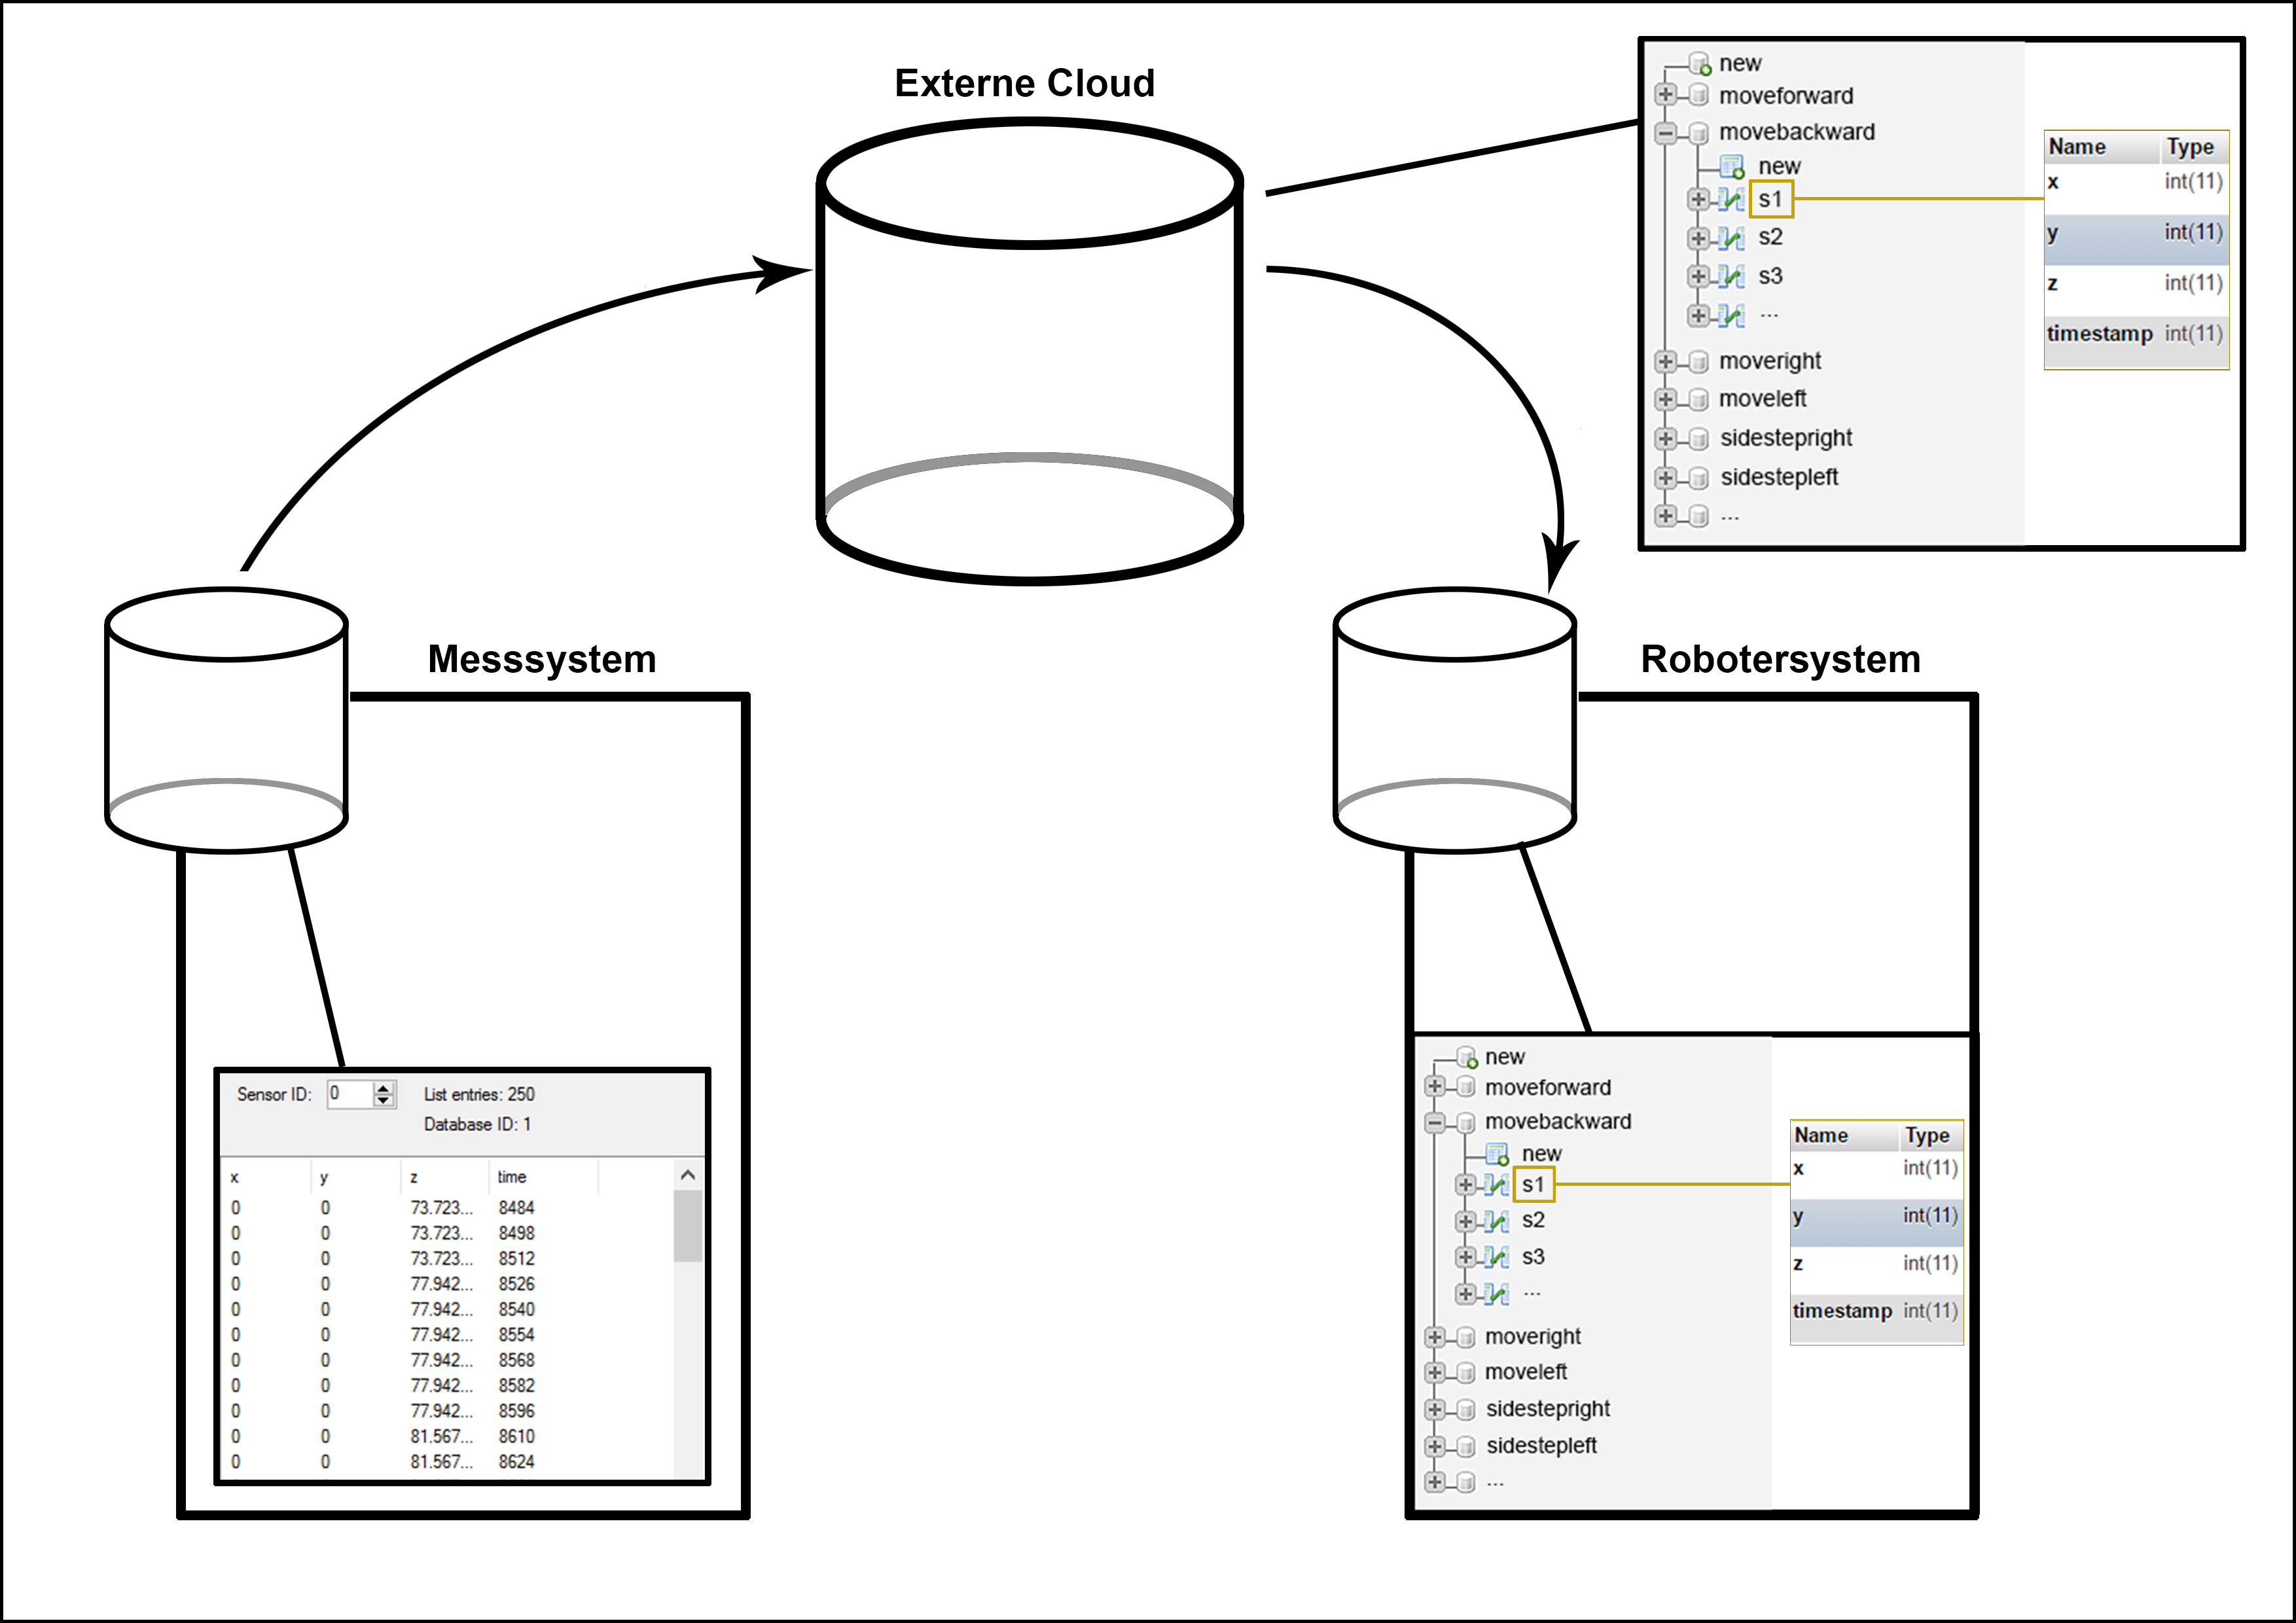
\includegraphics[width=1.0\linewidth]{03_Grafiken/DatabaseLayout/dblayout}
\caption[Layout der Datenbanken]{Layout der Datenbanken}
\label{fig:dblayout}
\end{figure}

Der oben dargestellte zylinderf�rmige Komponente repr�sentiert die externe Cloud, welche �ber das Internet erreichbar ist. Diese beinhaltet die Bewegungsdaten f�r alle Motoren, welche zuvor durch das Messsystem aufgenommen und extrahiert wurden. Die Struktur (s. seitlicher Bereich) besteht aus mehreren Datenbanken, von denen jede mehrere Tabellen enth�lt, in denen die Sensorwerte hinterlegt sind. Abbildung \ref{fig:cloudcontent} zeigt exemplarisch den Aufbau der Cloud.

\begin{figure}[H]
\centering
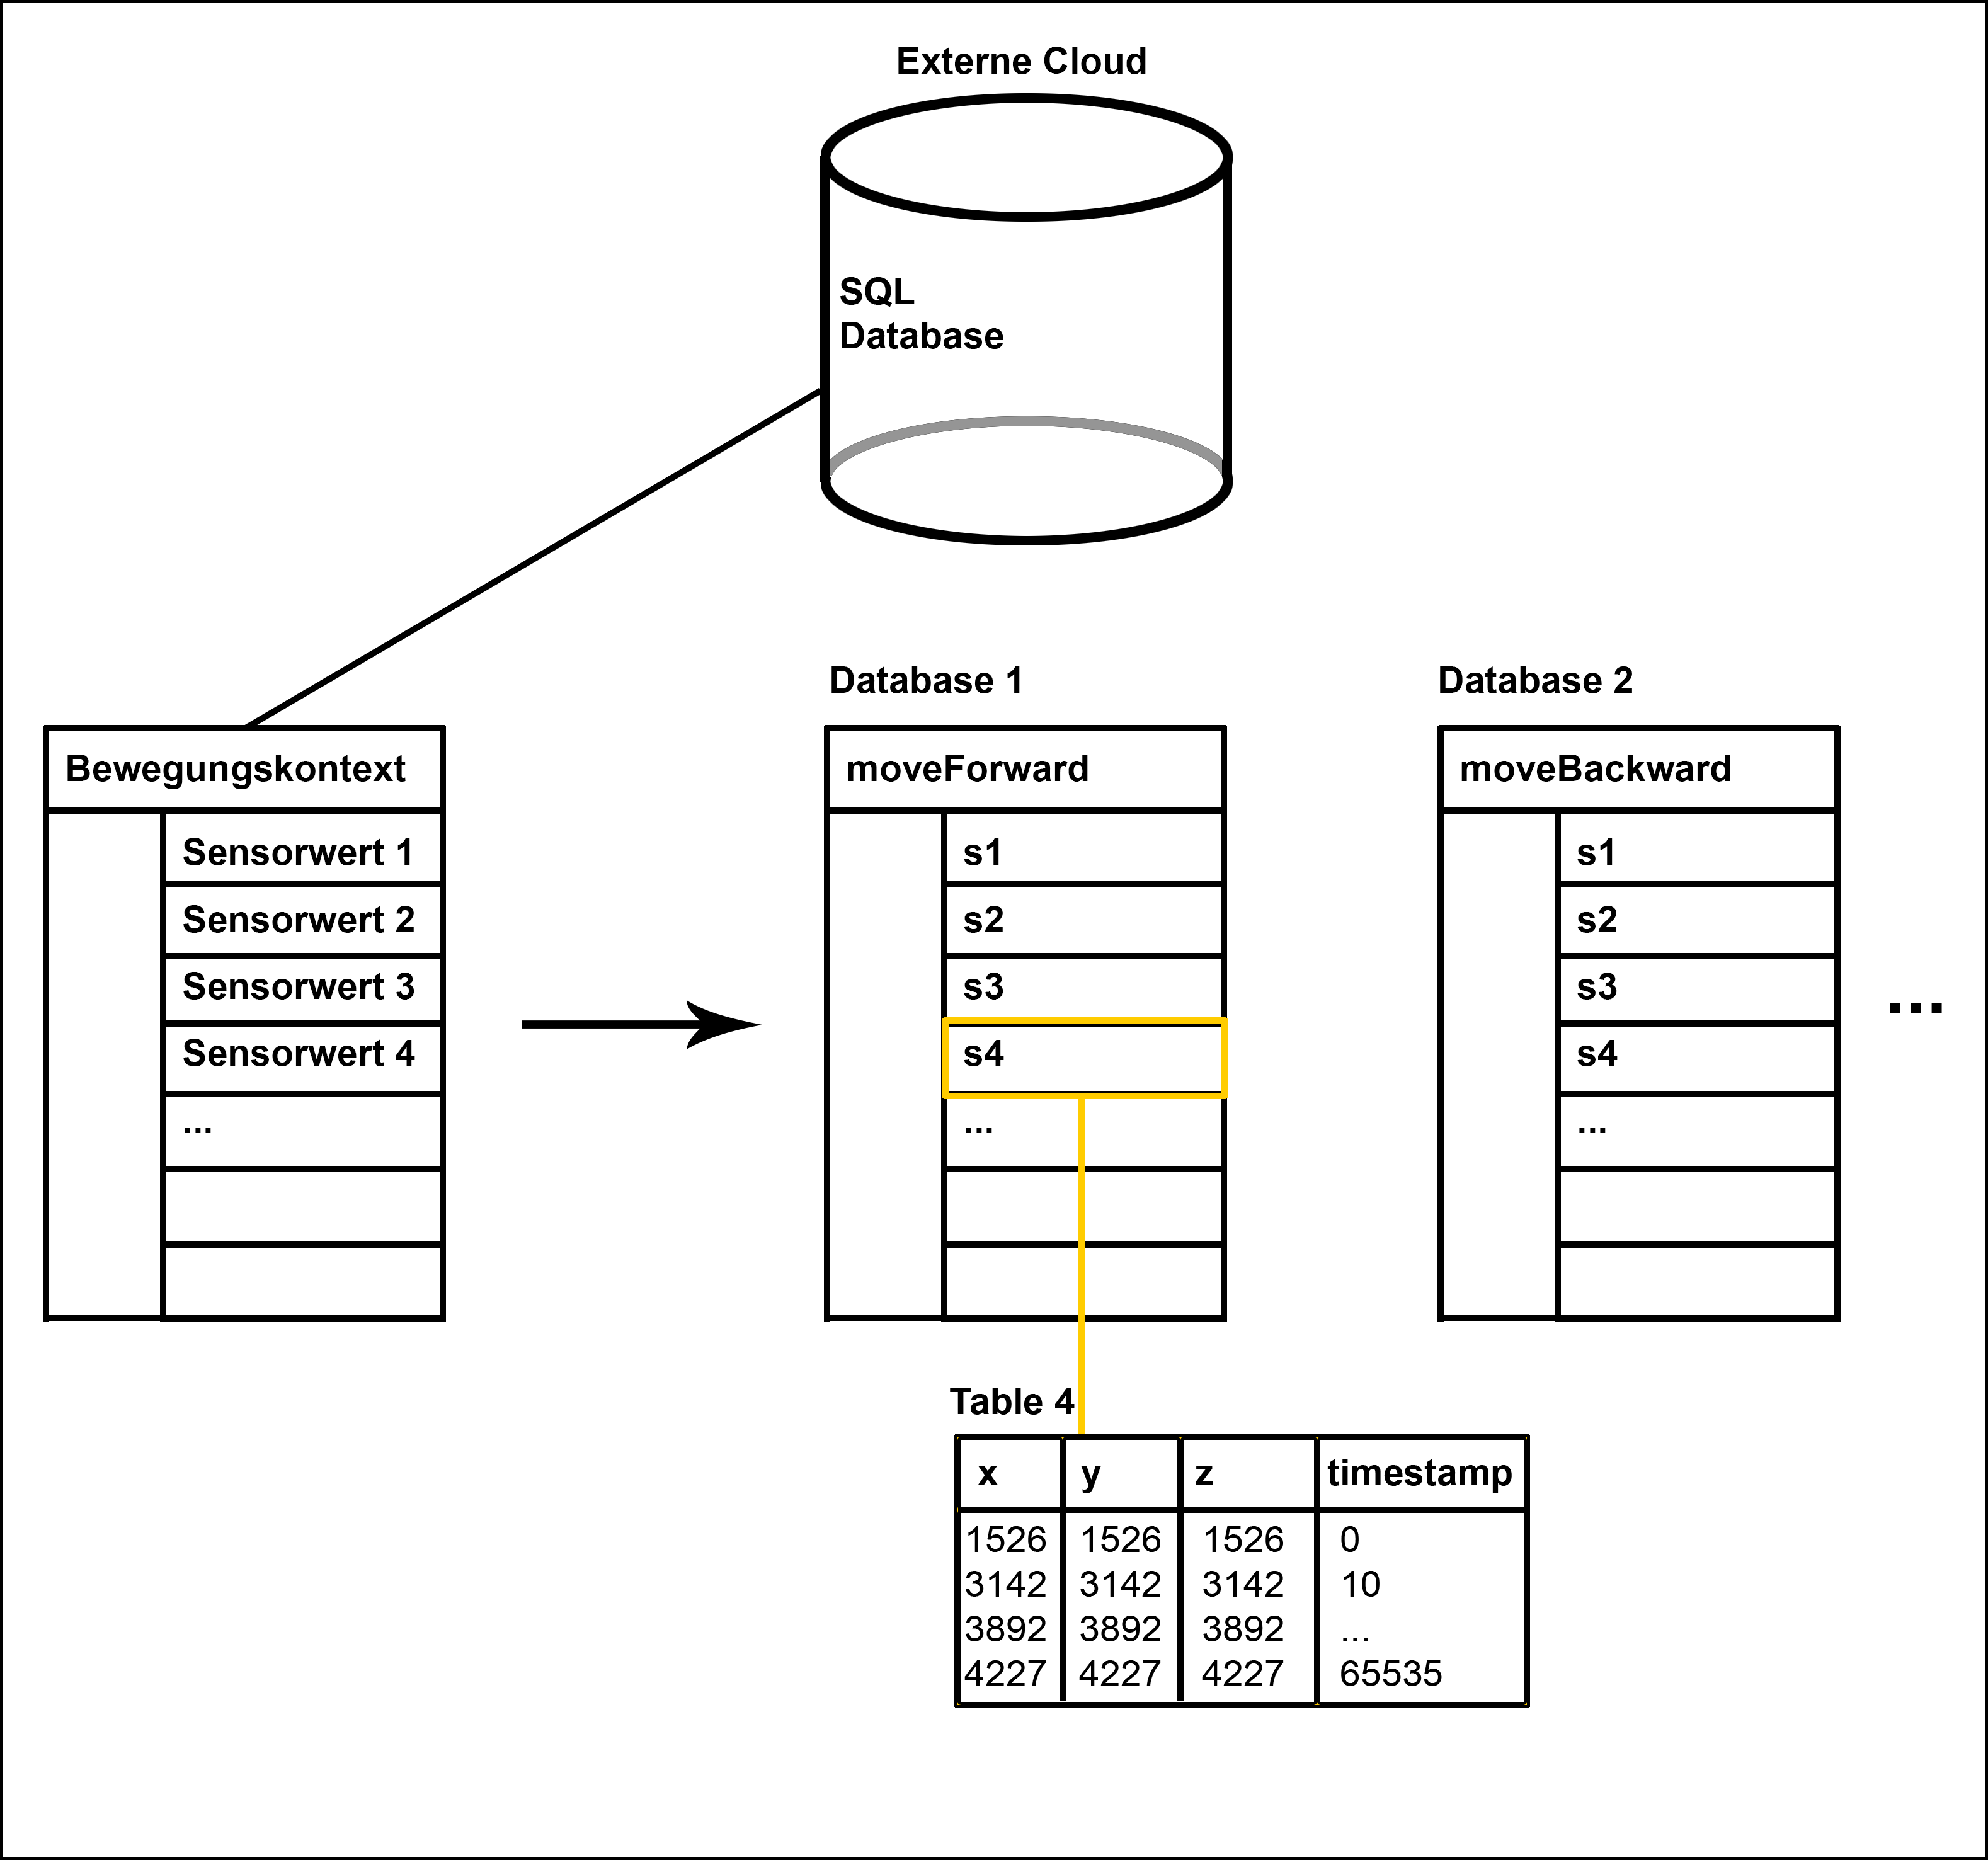
\includegraphics[width=1.0\linewidth]{03_Grafiken/DatabaseLayout/CloudContent}
\caption[Struktur der externen Cloud]{Struktur der externen Cloud}
\label{fig:cloudcontent}
\end{figure}

Die links dargestellte Komponente zeigt den grunds�tzlichen Aufbau einer Datenbank mit den darin liegenden Tabellen. Darin enthalten sind die Werte aller Sensoren in extrahierter Form, multipliziert mit dem Faktor 100. Die beiden rechts dargestellten Tabellen zeigen beispielhaft den Kontext der Datenbanken. Dieser ist mit der entsprechenden Bewegungsart definiert (z.B. Vorw�rtsgehen, R�ckw�rtsgehen, etc.). Unterhalb der beiden Tabellen wird der Inhalt einer Tabelle innerhalb einer Datenbank (z.B. Tabelle \textit{s4} in der Datenbank \textit{moveForward}) aufgezeigt. Dabei ist zu beachten, dass die Eintr�ge aus maximal 2 byte bestehen d�rfen, da das Protokoll mehr nicht zul�sst (s. Kapitel \ref{kap:Protokoll}). F�r die Sensorwerte ist dies irrelevant, da diese max. $ \alpha = 90 [deg]$, bzw. 9000 erreichen k�nnen. Wichtig ist dies allerdings f�r den Zeitstempel. Dieser kann max. 65535 erreichen, was eine Messdauer von ca. $ \Delta t = 60 [s]$ entspricht. F�r die grunds�tzliche Fortbewegung ist es ausreichend, f�r ganze Bewegungstasks (z.B. geskriptes Inlineskaten) jedoch nicht.

